\begin{figure*}
\caption{General architecture of an SLA guided  data integration system.\label{fig:arch}}
\end{figure*}

Figure~\ref{fig:arch} shows the general architecture of an SLA guided data integration system that is supported by data services which are data providers deployed in a cloud and that provide agreed SLA’s. 
These descriptions are stored in a directory together with meta-data about the way queries are evaluated for producing results. 
The system uses this information  by query processing and monitoring modules for rewriting queries according to given quality of service (QoS) preferences expressed by a data consumer, for example a user.


Consider a smart city that aims at being energy self-sustainable and produce and consume as much as possible, energy within its geographic area. 
Producers are characterized according to their location, the amount of energy in kWatts-hour that they can sell, the cost, and the time window in which they can produce it, with a given service level agreement concerning their availability and fault tolerance. 
Consumers, give also their location, their energy requirements during a certain interval of time, the maximum total cost they are ready to pay, and quality of service requirements such as availability and how critical it is to consume this amount of energy. 
A energy exchange market is established in order to continuously monitor energy provision/consumption ensuring that all consumers will have the energy they require at every moment.

\begin{figure*}
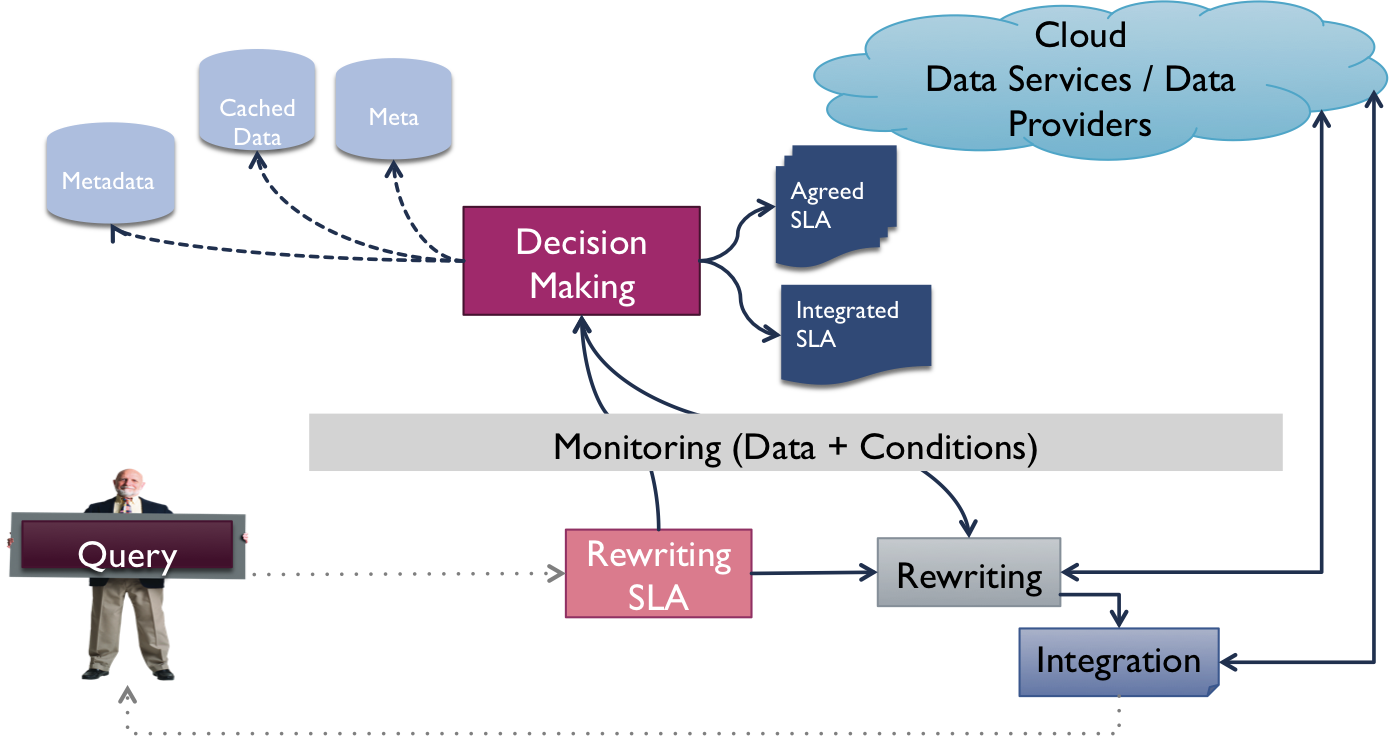
\includegraphics[width=0.6\textwidth]{figs/arch.png}
\caption{\label{fig:energyXChange} Energy exchange.}
\end{figure*}

In our approach energy producers are modelled as services with associated ``agreed'' SLAs for a given time window. 
In general, we assume that several producers will be able to supply energy for a given period of time given specific QoS preferences expressed by a consumer. 
An energy request is expressed as a query that specifies an energy requirement with QoS preferences independently of the possible producers. 

\begin{itemize}
\item Processing big data implied in the energy consumption observation 
\item Computing energy consumption behavior models
\item Analyse and optimize energy consumption versus respecting the comfort requirement of inhabitants
\end{itemize}

Need of efficient data processing solutions


 Given a query, expressed as an SQL like expression including spatio-temporal attributes and preferences, for example, {\em List of energy providers that can provision 1000 Kwatts/h, in the next 10 seconds, that are close to my city with a cost of 0,50 euros/Kwatt?}. Assuming also that energy providers are represented by services exporting their SLA agreements and that can potentially be combined for answering the query. 